\documentclass{article}

\usepackage{neurips_2026}

\usepackage[utf8]{inputenc}
\usepackage[T1]{fontenc}
\usepackage{hyperref}
\usepackage{url}
\usepackage{booktabs}
\usepackage{graphicx}
\usepackage{amsfonts}
\usepackage{amsmath}
\usepackage{nicefrac}
\usepackage{microtype}
\usepackage{xcolor}
\usepackage{algorithm}
\usepackage{algpseudocode}
\usepackage{multirow}
\usepackage{enumitem}

\title{DPGrammar: Joint Viterbi Repair for Grammar-Constrained\\Diffusion Language Models}

\author{%
  Anonymous Author(s)\\
  Affiliation\\
  Address\\
  \texttt{email}
}

\begin{document}

\maketitle

\begin{abstract}
Constrained decoding ensures LLM outputs follow structured formats like JSON, 
but existing systems rely on autoregressive, left-to-right parsing to mask invalid 
tokens. Diffusion language models break this paradigm by unmasking positions based 
on confidence rather than linear order. Because downstream tokens are already final by 
the time the parser reaches them, the grammar cannot be enforced ahead of the parse frontier; instead, it must be repaired 
behind it. Crucially, repairing one position at a time is insufficient because grammatical 
constraints couple multiple positions; a locally probable fix can easily eliminate 
all valid global completions. To address this, we present \textbf{DPGrammar}, a repair layer 
that resolves violations jointly over the affected span. By treating the parser state as a 
sufficient statistic to merge interchangeable search paths, DPGrammar executes a 
Viterbi pass over (parser state $\times$ position) pairs to find the global highest-likelihood 
valid assignment in polynomial time. Drawing candidates directly from the automaton's 
outgoing edges eliminates missed proposals by construction, while deriving termination 
conditions from the grammar removes empirical tuning constants. Evaluating with LLaDA-8B-Instruct 
on JSONSchemaBench \texttt{medium}, DPGrammar raises schema validity from $91.8\%$ to $96.7\%$ 
while cutting corrective overhead from $33.2$ to $1.2$ remasks per instance. 
Notably, our margin over the unrepaired baseline more than doubles to $10.3$\,pp 
once outputs are required to carry content, and reaches $+13.4$\,pp on the hardest 
split where joint violations dominate.
\end{abstract}

\section{Introduction}

% context
Masked diffusion language models (dLLMs) such as LLaDA-8B \citep{llada} and Dream-7B \citep{dream} generate by iteratively unmasking
positions in confidence order rather than left to right, decoding many tokens
per forward pass and trading sequential depth for parallelism. Some of the applications require
output that is structured, for example, an agent calling a tool needs JSON conforming to a given schema
\citep{patil2025bfcl,geng2025jsonschemabenchrigorousbenchmarkstructured}, and one
misplaced brace makes the response unusable to the caller no matter how good its
content. Autoregressive (AR) models meet this requirement through constrained
decoding: an incremental parser tracks the partial output and masks any next
token that would violate the grammar \citep{outlines}, machinery now standard in
serving frameworks \citep{dong2024xgrammar,guidance,zheng2024sglang,microsoft2025llguidance}.

% problem + prevention vs. repair
That machinery assumes commitment happens left to right, and a dLLM commits out
of order. At any decoding step the sequence comprises a validated prefix, a
frontier the parser constrains, and tokens the model has filled but the parser
has not read. Masked diffusion is \emph{carry-over unmasking}: a revealed
position is copied unchanged in every later step
\citep{sahoo2024simple,shi2024simplified}, so when the frontier reaches those
tokens the parser may reject one the decoder can no longer un-place. One solution is to prevent violations by making the
constraint globally tractable and sampling from the constrained posterior
exactly \citep{suresh2025dingoconstrainedinferencediffusion}. Prevention
guarantees satisfaction by construction, but it needs a regular representation,
and a recursive JSON Schema with unbounded nesting is not
regular.\footnote{On JSONSchemaBench \texttt{medium} an automata toolchain
compiles $383$ of $586$ schemas where an incremental context-free parser handles
$511$ (Table~\ref{tab:coverage}); a guarantee unavailable on a third of the
workload is not a guarantee for it.} It also pays
at every denoising step and fixes the decoding order, whereas repair costs
nothing on a clean step and leaves the schedule free. We therefore repair after
the fact, forgoing the certified guarantee. Existing repair, though, is myopic
\citep{zhang2026lookaheadthenverifyreliableconstraineddecoding,cd4dllm}: it
rewrites the position the parser rejected and leaves the rest of the region
alone. That is not enough, because a grammar couples the positions it
constrains: whether a token leads anywhere depends on what must follow it, so a
choice that is both locally probable and locally legal can still eliminate every
valid completion of the region. The model gives no signal about this, its
per-position distributions being independent where the grammar is not. A missing
brace, a key matching no property and a stray comma are then one error rather
than three, and the region has to be decided as a whole.

% method
To bridge this gap, we introduce \textbf{DPGrammar}, a repair layer that treats
a violated region as a single decision problem rather than a sequence of
independent ones. When the parser rejects at the frontier, we identify the
affected span and run a Viterbi search over a lattice of (parser state $\times$
position) pairs, selecting the highest-likelihood assignment for the whole span
that the grammar accepts. Deciding a region jointly would be exponential in its
length if the search ranged over token sequences. It does not, because the
parser state is a sufficient statistic for everything that follows: two paths
arriving at the same state are interchangeable from there on, so merging them
discards no optimum, and one Viterbi pass returns the exact maximiser in time
linear in the span. Candidates at each node come from the automaton
itself, the parser's outgoing edge set at that state, ranked by model
likelihood, which is the smaller object to search and the one that cannot miss a
legal token.\footnote{Against a vocabulary of $126{,}349$, a live parser state 
admits a median of just $106$ tokens (\S\ref{sec:cand}, Appendix~\ref{app:legalsets}).}
Termination is decided by the grammar rather than by a step count: we stop when
the parser has no choices left but to stop. Because this layer fires only after a 
rejection, it is agnostic to the unmasking schedule. Moreover, by delegating parsing 
to an off-the-shelf incremental parser \citep{microsoft2025llguidance}, it supports 
context-free constraints instead of being limited to regular ones.

% results
Empirically, we evaluate our approach on JSONSchemaBench \citep{geng2025jsonschemabenchrigorousbenchmarkstructured} and JSON-Mode-Eval \citep{nousresearch2024jsonmodeeval,ethsri2025jsonmodeevalextended} using LLaDA-8B-Instruct, benchmarking against LAVE, CD-CFG \citep{cd4dllm}, and an ablation variant with the
repair layer disabled. On $511$
\texttt{medium} instances, DPGrammar reaches $96.7\%$ schema validity against
$91.8\%$ with the layer off, and cuts mean repair events from $33.2$ to $1.2$.
Finally, the layer's benefit is not a constant offset but grows with the
density of joint constraints: across \texttt{easy}, \texttt{medium} and
\texttt{hard} the validity margin is $+0.2$, $+4.9$ and $+13.4$\,pp, and the
content margin $+4.1$, $+10.3$ and $+17.8$\,pp. On a grammar whose violations
are purely local the layer never fires at all, which places the same claim at
the other end of that axis.

\section{Related Work}

\paragraph{Constrained decoding for AR LLMs.}
Constrained decoding for AR LLMs relies on compiling grammars into incremental automata to mask invalid logits at each step \citep{outlines, dong2024xgrammar, microsoft2025llguidance}, with much of the recent work spent on making that mask cheap to compute: SynCode \citep{ugare2025syncode} precomputes a token-lexeme store, and \citet{park2025flexible} cut the offline preprocessing by an order of magnitude while matching online mask cost. Further extensions enforce semantic constraints \citep{poesia2022synchromesh} or type-system completability guarantees \citep{muendler2025typeconstrained}. Crucially, all such methods assume strict monotonic, left-to-right generation. The challenge of handling out-of-order token commitments never arises in AR decoding, yet it constitutes the central problem in dLLMs.

\paragraph{Constrained decoding for dLLMs.}
\citet{cd4dllm} propose CFG-constrained dLLM decoder, intersecting the
grammar with an automaton over the generated prefix. DINGO
\citep{suresh2025dingoconstrainedinferencediffusion} performs MAP inference over
a deterministic finite automaton weighted by the model's mean-field predictions,
and \citet{dang2026fadllm} generalise this to exact sampling from the
constrained mean-field posterior under arbitrary remasking schedules, restoring
a hard guarantee. Both require the constraint as a finite automaton, which
bounds them to regular languages; we trade that guarantee for a context-free
constraint language and a schedule-agnostic layer. LAVE
\citep{zhang2026lookaheadthenverifyreliableconstraineddecoding} verifies each
frontier token by sampling $K$ random completions, accepting only if one is
grammar-valid; it is the dominant published baseline. Plan-style decoders
\citep{li2026planverifyfillstructured} emphasise structure-aware planning. In contrast, we maintain a lightweight incremental parser at the token level, triggering joint search where parsing conflicts arise.

\paragraph{Viterbi decoding for non-AR models.}
Lattice search is well-established in non-autoregressive generation \citep{deng2021sequence}. For instance, \citet{shao2022viterbi} apply Viterbi decoding over Directed Acyclic Transformers, and Control-DAG \citep{chen2024controldag} enforces lexical constraints via Weighted Finite State Automata. Crucially, these methods search over a model-defined lattice where output length must be constrained to prevent unnormalized likelihoods from favoring trivially short paths. In contrast, our search lattice is defined by the parser and bounded by the violated span. Because length is fixed by the span rather than treated as a free search variable, objective-side heuristics, such as explicit edit penalties, have no impact on the final output (\S\ref{sec:ablation}).

\section{Method}
\label{sec:method}

\subsection{Problem statement}
\label{sec:problem}

Let $G$ be a grammar and let its \emph{incremental parser} be an object that processes tokens left to right. After accepting a prefix, the parser maintains a \emph{state} $q$ defining the valid continuations permitted by $G$. Write
$\mathcal{L}(q)\subseteq V$ for the set of tokens the parser can consume from
$q$, its outgoing edge set (Appendix~\ref{app:api} shows the concrete interface). The decoder holds a sequence $x$ over
$V\cup\{\textsc{mask}\}$; its frontier $c$ is the length of the longest
prefix the parser has consumed, and $q_c$ the state it reached there. 
Because unmasking follows confidence rather than position, the region beyond the frontier mixes masked slots with tokens the model has already placed:
\[
\underbrace{x_0\;\cdots\;x_{c-1}}_{\text{consumed, parser at }q_c}
\;\;\Big|\;\;
\underbrace{x_c}_{\text{frontier}}
\;\;\Big|\;\;
\underbrace{\textsc{mask}\;\;x_{c+2}\;\;\textsc{mask}\;\;x_{c+4}\;\;\cdots}_{\text{placed but never parsed}}
\]
Only $x_c$ is under the parser's control: frontier masking guarantees
$x_c\in\mathcal{L}(q_c)$ when $x_c$ is chosen this step, while every position to
its right was sampled with no constraint at all.

Those positions are not provisional. Masked diffusion is \emph{carry-over
unmasking} \citep{sahoo2024simple,shi2024simplified}: the reverse posterior
copies any already-revealed position unchanged, so a step only ever replaces
$\textsc{mask}$ symbols,
\[
x_0 \;\leftarrow\; \mathbf{1}[\text{mask}]\odot x_0 \;+\; (1-\mathbf{1}[\text{mask}])\odot x ,
\]
which is what LLaDA's reference sampler implements. (Samplers that deliberately
remask revealed positions relax the property; we do not assume one.) Tokens
placed beyond the frontier are therefore immutable commitments. As remaining masks fill in, the parser advances across the newly contiguous region and may eventually encounter a position $v>c$ where $x_v\notin\mathcal{L}(q_v)$. We define $v$ as a \emph{violator}: a final, unalterable token that the grammar refuses.

\paragraph{Why this is challenging.}
% 改單一位置通常沒用,因為造成違規的 token 可能在好幾個位置之外
Every constrained decoder for autoregressive models is a filter: it inspects the
distribution at one position and removes what the grammar forbids. Positioned past the frontier, a violator cannot be filtered; it must be overwritten. Yet, local repair rarely works, because the interacting tokens that cause the violation are often several positions away. The problem is therefore a \emph{search} over joint assignments
to a region, not a filter over a single distribution.

\subsection{Repair as bounded search}

Figure~\ref{fig:pipeline} in Appendix~\ref{app:pipeline} places the layer in the
loop it runs inside; this section describes what it does once a rejection
reaches it. Given a violator $v$, the layer repairs a bounded span $[v,e)$ with
$e=\min(v+L,\;\text{first }\textsc{mask})$ and $L$ a compute budget: it rewrites
committed positions and never fills holes. Over that span we seek the assignment
$y$ maximising $\sum_{p}\log p_\theta(y_p\mid x)$ subject to the parser
accepting $y_v\cdots y_{e-1}$ from $q_v$. This is a shortest-path problem on a
layered graph whose nodes are (position, parser state) pairs and whose edges out
of a state are exactly $\mathcal{L}(q)$.

When the parser rejects at $v$, the decoder tries, in order:

\begin{enumerate}[leftmargin=1.4em,itemsep=1pt,topsep=2pt]
\item \textbf{Termination check.} If the parser cannot consume anything, or the
      model has placed a stop token at the frontier and the parser permits
      stopping, the document ends (\S\ref{sec:stop}).
\item \textbf{Single-token retry.} Walk the model's ranked logits at $v$ for up
      to $10$ candidates and take the first the parser accepts. This is
      filter-then-propose, the pattern \S\ref{sec:cand} argues against, but here
      a miss is free: the position simply falls through to the joint search below. It resolves
      $62\%$ of violations at negligible cost.
\item \textbf{Joint DP repair.} Otherwise solve the span $[v,e)$ jointly
      (\S\ref{sec:dp}).
\item \textbf{Hand back.} If no assignment exists, remask $v$ and let the sampler
      re-derive it.
\end{enumerate}

Two design choices decide if the search is sound: which nodes it expands (\S\ref{sec:cand}), and when it is allowed to
stop (\S\ref{sec:stop}).

\subsection{Joint repair by Viterbi over parser states}
\label{sec:dp}

Algorithm~\ref{alg:dp} gives the search. It is a Viterbi pass over layers
indexed by position, where a node is a reachable \emph{parser state} rather than
a token history. We merge candidates who leave the parser in the
same state $\kappa'$ collapse to the single highest-scoring path (shown in line 11). It is exact
rather than a pruning heuristic, because the state determines every later
decision and a discarded path could never have overtaken the one kept. It is
also what bounds the search. Enumerating assignments over the span keeps
$O(k^{\text{span}})$ hypotheses alive; merging caps each layer at the number of
reachable parser states $|S|$, giving $O(\text{span}\cdot|S|\cdot k)$ parser
operations and $O(|S|)$ live parsers. The key
$\kappa(q)=\texttt{bytes}(\mathcal{L}(q))$ is the parser's own mask, which
line~5 already computed to build $C$, so the merge costs no parser call of its
own. Since $|S|$ stays in the single digits in
practice, span length stops being an exponent in either time or memory.

\begin{algorithm}[t]
\caption{Joint repair of a violated span}
\label{alg:dp}
\begin{algorithmic}[1]
\Require violator $v$, span end $e$, parser state $q_v$, log-probabilities
$\log p_\theta$, candidate budget $k$
\Ensure an assignment over $[v,e')$, $e'\!\le\!e$, that the parser accepts from $q_v$
\State $S \gets \{\,\kappa(q_v)\mapsto(q_v,\,0)\,\}$ \Comment{state key $\mapsto$ (parser, score)}
\For{$p = v$ \textbf{to} $e-1$}
  \State $W \gets \emptyset$ \Comment{best incoming path per successor state}
  \ForAll{$(q,s) \in S$}
    \State $C \gets \text{the } k \text{ most probable tokens of } \mathcal{L}(q)\setminus\{\textsc{eos}\}$ \Comment{\S\ref{sec:cand}}
    \State $C \gets C \cup \{x_p\}$ if $x_p \in \mathcal{L}(q)$ \Comment{keep the model's own token reachable}
    \ForAll{$t \in C$}
      \State advance $q$ by $t$; \; $\kappa' \gets \kappa(q)$; \; $s' \gets s + \log p_\theta(t)_p$
      \State \textbf{rollback} $q$ one token \Comment{probe without copying}
      \If{$\kappa' \notin W$ \textbf{or} $s' > \operatorname{score}(W[\kappa'])$}
        \State $W[\kappa'] \gets (q,\,t,\,s')$ \Comment{\textbf{merge}: paths reaching $\kappa'$ collapse to the best one}
      \EndIf
    \EndFor
  \EndFor
  \If{$W = \emptyset$}
    \State \textbf{break} \Comment{nothing consumable: the span ends here, it does not fail}
  \EndIf
  \State $S \gets \{\,\kappa' \mapsto (\textbf{clone}(q)\text{ advanced by }t,\; s') \;:\; (\kappa',(q,t,s')) \in W\,\}$
\EndFor
\State \Return the backtrace from $\arg\max_{q\in S}\operatorname{score}(q)$
\end{algorithmic}
\end{algorithm}

\subsection{Candidates from the automaton}
\label{sec:cand}

At each lattice node the search needs a set of tokens to try. We draw it from
the parser rather than from the model: for a live state $q$ we read
$\mathcal{L}(q)$, the tokens that state can consume, and rank \emph{within} it
by model likelihood,
\begin{equation}
\label{eq:cand}
\mathcal{C}(q,p) \;=\; \operatorname*{top-}k_{\,t\,\in\,\mathcal{L}(q)\setminus\{\textsc{eos}\}}\; \log p_\theta(t\mid x,p).
\end{equation}

The alternative is to rank the model's top-$k$ over $V$ and keep whichever
tokens the parser accepts. That is rejection sampling against
$\mathcal{L}(q)$, whose size is a property of the grammar rather than a
hyperparameter, so no choice of $k$ removes the risk: where the admitted set is
small the draw misses it entirely, and the DP then reports ``no path'' at a
position where one exists.

Drawing from $\mathcal{L}(q)$ removes that failure mode by construction, because
the proposal \emph{is} the accepted set. The search therefore keeps the property
the repair layer depends on: it returns the best assignment the grammar accepts
whenever one exists, instead of sometimes failing to find one that does. Where
$|\mathcal{L}(q)|\le k$ the edge set is enumerated exactly rather than sampled,
making the search at those nodes exhaustive rather than heuristic, and the only
cost is one mask read per (state, position), which the implementation already
paid to compute state keys. $\mathcal{C}$ is empty only where the grammar admits
nothing but a stop token, in which case the document is finished and there is
nothing to place. Appendix~\ref{app:legalsets} measures how often the two orders
diverge and what reversing them costs.

\subsection{Termination as a grammar question}
\label{sec:stop}

Termination cannot be left to the parser: \textsc{eos} is not a consumable
grammar symbol, so a finished document reaches the frontier looking exactly like
a violation. The repair layer tells the two apart before it does anything else,
by separating two questions:
\begin{itemize}[leftmargin=1.4em,itemsep=1pt,topsep=2pt]
\item \emph{The harness ends the document} only when
      $\mathcal{L}(q)\setminus\{\textsc{eos},\textsc{eot}\}=\emptyset$ and $q$ is
      accepting: the parser has no alternative, so ending is not a choice anyone
      is making.
\item \emph{The model ends the document} when it places a stop token at the
      frontier and $q$ is accepting: the model has asked, and the grammar need
      only permit it.
\end{itemize}
Both conditions are read off the grammar rather than from a step budget, so how
long an output should be is decided by the model and the grammar rather than by
the harness.

\subsection{System optimisations}
The repair layer sits on a frontier-constrained decoder, and the latencies we
report depend on how that decoder avoids redundant work. Parser work is not
repeated: one incremental parser is
carried across denoising steps rather than re-parsing the prefix each time, and
the search probes candidates by advancing and rolling back, so a parser is
copied only for states that survive. Model work is not repeated either:
resampling reuses the logits already in hand instead of a fresh forward pass,
and committed tokens are batched with an additive-increase schedule so that
clean stretches advance several positions per step. Finally, mask construction
for the next position overlaps the current forward pass, keeping the parser off
the critical path.

\paragraph{What the no-DP baseline is.}
Every comparison labelled ``no-DP baseline'' is \emph{the same binary, the same
checkpoint, the same schedule, and the same seed, with the DP layer switched
off}. On a violation it keeps the bounded single-token retry and, when that is
exhausted, hands the position back to the sampler; the joint search never runs.
Nothing else differs. We report it this way rather than as a separate system so
that the difference between the two columns is attributable to the repair layer
alone, and not to any of the engineering above, which both columns share.

\section{Experiments}
\label{sec:metric}

\subsection{Setup and metrics}

\paragraph{Datasets.}
JSONSchemaBench~\citep{geng2025jsonschemabenchrigorousbenchmarkstructured}
supplies JSON schemas without reference answers, in three difficulty splits:
\texttt{easy} and \texttt{medium} ($586$ instances each) and \texttt{hard}
($368$). Schemas that \textsc{llguidance} cannot compile are excluded from every
arm, since no method runs on them: $28$, $75$, and $99$ respectively, leaving
$n=558$, $511$, $269$. JSON-Mode-Eval supplies prompts paired with a schema \emph{and} a reference
completion; we use the $272$-instance extension
\citep{ethsri2025jsonmodeevalextended} of the original $100$-row
release~\citep{nousresearch2024jsonmodeeval}, as released with CD-CFG.

\paragraph{Models.}
All arms run LLaDA-8B-Instruct~\citep{llada} with $T{=}128$ denoising steps,
generation length $256$, block length $32$, and temperature $0.2$, on a single
A100 per shard. Grammars are compiled by
llguidance~\citep{microsoft2025llguidance} except where noted.

\paragraph{Baselines.}
\emph{Vanilla} is the same decoder with no constraint of any kind, and marks
what the backbone produces unaided. \emph{CD-CFG} \citep{cd4dllm} is run from the
authors' released implementation, which builds its constraint with
\textsc{rustformlang}, the formal-language library that ships with it; \S\ref{sec:coverage}
treats the resulting coverage difference separately. \emph{LAVE}
\citep{zhang2026lookaheadthenverifyreliableconstraineddecoding} is likewise run
from its authors' released code, instrumented only to record per-operation
timing, under a $120$\,second per-instance cap.
\emph{no-DP} is our own system with the repair layer switched off, as defined in
\S\ref{sec:method}.

% no-need
% We compare against the decoders we can run on the same backbone at the same
% expressiveness. DINGO
% \citep{suresh2025dingoconstrainedinferencediffusion} and the exact-sampling
% method of \citet{dang2026fadllm} are the closest work we do not run: both take
% the constraint as a finite automaton, so comparison would first
% require compiling each JSON Schema to a DFA, which is not possible for the
% recursive schemas in these splits and would confound their algorithm with that
% translation on the rest. We also found no released implementation of either at
% the time of writing. Their guarantee is therefore reported as a property of
% those methods rather than measured here.

\paragraph{Metrics.}
We report three quality metrics:
\begin{itemize}[leftmargin=1.4em,itemsep=1pt,topsep=2pt]
\item \emph{schema@1}: the output validates against the instance's own schema
      under \texttt{jsonschema}.
\item \emph{content}: it validates \emph{and} carries at least five scalar
      leaves. A schema is satisfied by the smallest document it permits, so
      validity alone scores an empty structure as a success and cannot separate
      it from a populated one; Appendix~\ref{app:example} shows a pair the two
      metrics order differently, and Table~\ref{tab:main} sweeps the threshold.
\item \emph{functional@1}: it matches the reference completion. JSON-Mode-Eval
      only, since JSONSchemaBench supplies no reference answer.
\end{itemize}
and two cost metrics: corrective work per instance (\emph{rs/inst}, whose unit
differs by arm and is defined with Table~\ref{tab:difficulty}) and wall-clock
latency, reported as mean, p50, p95 and p99 with timeouts at a $120$\,s cap.

\subsection{Main results}
\label{sec:results}

\begin{table}[t]
\centering
\small
\setlength{\tabcolsep}{4pt}
\caption{The difficulty gradient on LLaDA-8B-Instruct. Each arm is scored on
the instances its own toolchain compiles, so $n$ differs: LAVE, no-DP and DPG
share the \textsc{llguidance} set exactly, while $\dagger$ marks CD-CFG, whose
\textsc{rustformlang} front-end accepts a smaller subset (Appendix~\ref{sec:coverage}). 
schema@1 validates against the instance's schema;
content additionally requires five populated leaves; times are seconds and TO
counts the $120$\,s cap. rs/inst is corrective work per instance, but its unit
differs by arm (remasks, lookahead draws, rejected candidates), so only no-DP
and DPG compare there. DPG is DPGrammar.}
\label{tab:difficulty}
\begin{tabular}{llrrrrrrrrr}
\toprule
Split & Method & $n$ & schema@1\,$\uparrow$ & content\,$\uparrow$ & mean\,$\downarrow$ & p50\,$\downarrow$ & p95\,$\downarrow$ & p99\,$\downarrow$ & TO\,$\downarrow$ & rs/inst\,$\downarrow$ \\
\midrule
\multirow{5}{*}{\texttt{easy}}
 & Vanilla           & $577$ & $62.9$ & $30.2$ & $8.34$  & $8.37$  & $11.23$  & $14.98$  & $0$ & --- \\
 & CD-CFG$^\dagger$  & $449$ & $56.3$ & $28.1$ & $6.22$  & $6.72$  & $11.54$  & $15.98$  & $0$ & $49.2$ \\
 & LAVE              & $558$ & $80.1$ & $40.5$ & $30.63$ & $6.71$  & $120.01$ & $120.01$ & $94$ & $207.3$ \\
 & no-DP (ours)      & $558$ & $97.5$ & $45.2$ & $7.58$  & $7.58$  & $\mathbf{11.47}$ & $\mathbf{15.09}$ & $\mathbf{0}$ & $20.7$ \\
 & DPG (ours)        & $558$ & $\mathbf{97.7}$ & $\mathbf{49.3}$ & $\mathbf{5.31}$ & $\mathbf{3.40}$ & $15.11$ & $29.06$ & $\mathbf{0}$ & $\mathbf{0.6}$ \\
\midrule
\multirow{5}{*}{\texttt{medium}}
 & Vanilla           & $586$ & $49.8$ & $47.1$ & $14.89$ & $14.36$ & $21.82$  & $31.67$  & $0$ & --- \\
 & CD-CFG$^\dagger$  & $383$ & $44.1$ & $41.0$ & $22.71$ & $14.16$ & $112.24$ & $120.00$ & $19$ & $57.3$ \\
 & LAVE              & $511$ & $78.3$ & $74.0$ & $38.50$ & $25.70$ & $120.00$ & $120.01$ & $60$ & $253.5$ \\
 & no-DP (ours)      & $511$ & $91.8$ & $74.6$ & $\mathbf{13.45}$ & $\mathbf{13.40}$ & $\mathbf{21.43}$ & $\mathbf{29.99}$ & $\mathbf{0}$ & $33.2$ \\
 & DPG (ours)        & $511$ & $\mathbf{96.7}$ & $\mathbf{84.9}$ & $16.75$ & $15.05$ & $36.21$ & $63.24$ & $\mathbf{0}$ & $\mathbf{1.2}$ \\
\midrule
\multirow{5}{*}{\texttt{hard}}
 & Vanilla           & $368$ & $20.7$ & $20.4$ & $44.64$ & $35.43$ & $103.48$ & $120.00$ & $4$ & --- \\
 & CD-CFG$^\dagger$  & $245$ & $11.4$ & $10.6$ & $57.61$ & $41.53$ & $120.00$ & $120.15$ & $72$ & $50.2$ \\
 & LAVE              & $269$ & $39.8$ & $39.4$ & $40.47$ & $38.35$ & $120.00$ & $120.00$ & $30$ & $115.8$ \\
 & no-DP (ours)      & $269$ & $74.3$ & $53.9$ & $\mathbf{31.41}$ & $\mathbf{26.69}$ & $\mathbf{61.91}$ & $\mathbf{101.51}$ & $\mathbf{0}$ & $56.0$ \\
 & DPG (ours)        & $269$ & $\mathbf{87.7}$ & $\mathbf{71.7}$ & $42.66$ & $35.24$ & $96.58$ & $115.96$ & $2$ & $\mathbf{1.5}$ \\
\bottomrule
\end{tabular}
\end{table}

\begin{table}[h]
\centering
\small
\caption{JSONSchemaBench \texttt{medium} ($n{=}511$) as the content floor
rises. Each row requires validity \emph{and} at least $\kappa$ populated leaves.}
% The two $\Delta$ columns have opposite shapes: our margin over the unrepaired
% baseline more than doubles once any content is required, while our margin over
% LAVE shrinks.}
\label{tab:main}
\begin{tabular}{lrrrrr}
\toprule
 & LAVE & no-DP & \textbf{DPGrammar} & $\Delta$ vs no-DP & $\Delta$ vs LAVE \\
\midrule
validity only        & $78.3$ & $91.8$ & $\mathbf{96.7}$ & $+4.9$  & $+18.4$ \\
$\wedge\ \kappa{=}1$  & $78.3$ & $84.9$ & $\mathbf{93.7}$ & $+8.8$  & $+15.4$ \\
$\wedge\ \kappa{=}3$  & $76.7$ & $79.1$ & $\mathbf{90.6}$ & $\mathbf{+11.5}$ & $+13.9$ \\
$\wedge\ \kappa{=}5$  & $74.0$ & $74.6$ & $\mathbf{84.9}$ & $+10.3$ & $+10.9$ \\
$\wedge\ \kappa{=}10$ & $56.0$ & $50.7$ & $\mathbf{60.5}$ & $+9.8$  & $+4.5$ \\
$\wedge\ \kappa{=}15$ & $33.7$ & $29.5$ & $\mathbf{35.0}$ & $+5.5$  & $+1.3$ \\
\bottomrule
\end{tabular}
\end{table}

Table~\ref{tab:difficulty} divides the experimental arms by what they do when enforcement fails. Two of the grammar-enforcing methods achieve validity levels that the unconstrained decoder cannot approach; CD-CFG does not, scoring below Vanilla at every tier even on the subset its own front-end compiles, which Appendix~\ref{sec:coverage} takes up rather than reading as a verdict on its decoding. LAVE discards and resamples blocks upon failure, which exhausts the full $120$\,s budget on $60$ \texttt{medium} and $94$ \texttt{easy} instances. In contrast, DPGrammar and the ablation baseline (no-DP) repair in place, and between them lose two instances to the cap across all three splits. Between these two, the control is tightly managed: activating the repair layer improves \texttt{medium} validity by $4.9$\,pp while cutting corrective overhead from $33.2$ to $1.19$ remasks per instance, costing a mere $3.3$\,s of mean wall time.

That headline understates the layer, because validity is satisfied by the
smallest document a schema permits and the unrepaired baseline often emits one.
Raising the content floor separates the two routes: our margin over no-DP more
than doubles once any content is required and holds near ten points to
$\kappa{=}10$ (Table~\ref{tab:main}). The mechanism is that single-token repair
takes the cheapest legal token at a violation, and a closing bracket usually is
one, so the document collapses where the joint solve continues it;
Appendix~\ref{app:example} shows an instance where both arms validate and only
the content floor tells them apart. Against LAVE the shape inverts, from
$18.4$ to $1.3$\,pp, because LAVE never repairs and its surviving documents were
never rewritten. Against LAVE we buy frequency; against the unrepaired baseline
we buy content.


We also looked into where the layer's extra wall time goes and found that the
bottleneck is not the search but the decoding it makes possible. The constraint
machinery costs what the baseline's does. What grows is everything downstream of
it, since a repaired document keeps going and takes $1.5\times$ the forward
passes to write $1.7\times$ the tokens (Appendix~\ref{app:workload}). The layer
is $3.3$\,s slower on average, but only where it fires: on the two thirds of
instances it never touches it is $1.1$\,s faster.

\paragraph{The margin grows with difficulty.}
% 差距隨難度單調成長,而且兩個指標都是,證實了「效益取決於違規有多聯合」
The margin grows with difficulty on both metrics: schema@1 by $+0.2$, $+4.9$ and
$+13.4$\,pp across \texttt{easy}, \texttt{medium} and \texttt{hard}, and content
by $+4.1$, $+10.3$ and $+17.8$\,pp. This is the pattern joint repair predicts,
since violations become more joint as schemas acquire nesting, required-property
ordering and cross-field constraints.

\paragraph{One class of violation the layer cannot repair.}
Not every residual failure is a failure of the search. \textsc{llguidance} pins
an object's properties to their declaration order, so a model that writes them
in a different order produces a violation that \texttt{jsonschema} would not
call an error at all, and whose correct repair is a movement rather than a
substitution, which a positional DP cannot express. This accounts for $7.6\%$ of
$118$ violations and for half of the $16$ that arise where the grammar admits
exactly one token (Appendix~\ref{app:ordering}). It is a limit of overwriting in
place rather than of solving the span jointly.

\subsection{Where correctness can be scored: JSON-Mode-Eval}
\label{sec:jme}

JSON-Mode-Eval pairs each prompt with a reference completion, so structural and
semantic correctness can be read apart.

\begin{table}[h]
\centering
\small
\caption{JSON-Mode-Eval, $n{=}272$, LLaDA-8B-Instruct. schema@1 is validity against the instance's schema, the same quantity as in
Table~\ref{tab:difficulty}; functional@1 additionally requires the output to
match the reference completion.}
\label{tab:jme}
\begin{tabular}{lrr}
\toprule
Method & schema@1\,$\uparrow$ & functional@1\,$\uparrow$ \\
\midrule
Vanilla    & $85.3\%$ & $48.6\%$ \\
CD-CFG      & $92.6\%$ & $52.6\%$ \\
LAVE       & $\mathbf{98.1\%}$ & $\mathbf{53.7\%}$ \\
no-DP      & $97.4\%$ & $\mathbf{53.7\%}$ \\
DPGrammar  & $\mathbf{98.1\%}$ & $52.6\%$ \\
\bottomrule
\end{tabular}
\end{table}

Grammar constraints buy structure and not semantics. Every constrained arm gains
$7$ to $13$\,pp of schema validity over Vanilla while functional@1 stays
within a $5$\,pp band, and inside that band our repair layer costs
$1.1$\,pp against leaving it off. A well-formed document is not a correct one,
and rewriting tokens to make it well-formed can move it away from the answer.

\subsection{Ablations: the objective does not matter, the search space does}
\label{sec:ablation}

\begin{table}[h]
\centering
\small
\caption{Ablation of the repair layer's components. The lower block lists
knobs that measure to exactly zero.}
\label{tab:ablation}
\begin{tabular}{llc}
\toprule
Component & Varied & Measured effect \\
\midrule
Candidate source     & vocabulary top-$k$ $\to$ automaton & schema@1 $95.5\to96.7$; proposal misses $4\to0$ \\
Repair window        & single token $\to$ full span       & 1-char leaves $12.3\%\to7.9\%$ \\
\midrule
Objective            & $\log p$ $\to$ min-edit            & $-0.5$ edits, $93.9\%$ identical \\
Candidate admission  & always admit committed token       & none (identical output) \\
Stop tokens          & excluded $\to$ kept in $\mathcal{C}$ & none; $48\times$ more futile probes \\
Post-hoc enrichment  & on $\to$ off                       & none (identical output) \\
Edit penalty & $\lambda\in\{0,2\}$ & none (never non-zero) \\
\bottomrule
\end{tabular}
\end{table}

We vary one component at a time against the reported configuration, holding the
backbone, seed and schedule fixed, on JSONSchemaBench \texttt{medium}.
Table~\ref{tab:ablation} gives the result: two components move the metric and
five do not, and the split falls along what each one touches. Both of the
former change what the search ranges over, and all of the latter are objective
terms or admission rules.

The candidate source carries one effect the aggregate hides. Ranking the
vocabulary and filtering costs $1.2$\,pp, but it also produces four repair sites
where the top-$k$ draw contained no token the parser would accept; the edge set
produced none in $315$ sites and cannot, being defined as what the parser
accepts. Among the inert components, minimum-edit leaves $93.9\%$ of outputs
byte-identical and attributes $90\%$ of what the DP rewrites to the grammar
rather than to the objective, and an explicit edit penalty never becomes
non-zero although it is the correction Viterbi decoders for non-autoregressive
models need to stop an unnormalised objective collapsing toward short
paths~\citep{shao2022viterbi,chen2024controldag}: our span is fixed by the
violation rather than chosen by the search, so there is no collapse to prevent.
Changing what the search optimises cannot help; changing what it searches over
can.

\section{Conclusion}

We present DPGrammar, a repair layer for grammar-constrained decoding in
diffusion language models, which commit tokens out of order and can therefore
only repair a violation after the fact. Casting that repair as a dynamic program
over parser states lets a violated region be decided as a whole and exactly
rather than one position at a time, since the state is a sufficient statistic
for what follows and paths reaching it merge without discarding the optimum.
What this achieves is validity held at the smallest intervention the grammar
allows. The search fires only after a rejection, proposes only tokens the parser
admits, follows the model's own ranking wherever the grammar leaves a choice,
and overwrites a position only where it does not.

\section{Limitations and future work}
\label{sec:limits}

Our results are one backbone and one seed on JSON, and the layer earns nothing
where violations are local rather than joint, as on SMILES, where the DP seldom fired. 
Testing other dLLM backbones, and other constraint families would establish where between those grammars and JSON Schema the layer begins to pay.
A more fundamental direction is the parser itself. We build on one written for
left-to-right decoding, which is why the constraint can be enforced at a single
frontier and everything past it can only be repaired. A checker designed for
dLLMs, tracking several disconnected regions at once, would let the grammar be
enforced at every region a step touches rather than at the leftmost one alone,
and would give a joint repair more of the sequence to work with.

\clearpage
\begin{thebibliography}{25}
\providecommand{\natexlab}[1]{#1}
\providecommand{\url}[1]{\texttt{#1}}
\expandafter\ifx\csname urlstyle\endcsname\relax
  \providecommand{\doi}[1]{doi: #1}\else
  \providecommand{\doi}{doi: \begingroup \urlstyle{rm}\Url}\fi

\bibitem[Chen et~al.(2024)Chen, Lin, Mei, and Byrne]{chen2024controldag}
Jinghong Chen, Weizhe Lin, Jingbiao Mei, and Bill Byrne.
\newblock Control-{DAG}: Constrained decoding for non-autoregressive directed
  acyclic {T5} using weighted finite state automata.
\newblock In \emph{Proceedings of the 2024 Conference of the North American
  Chapter of the Association for Computational Linguistics: Human Language
  Technologies (Short Papers)}, 2024.

\bibitem[Dang and Ermon(2026)]{dang2026fadllm}
Meihua Dang and Stefano Ermon.
\newblock Constrained decoding for diffusion language models via efficient
  inference over finite automata.
\newblock \emph{arXiv preprint arXiv:2607.07026}, 2026.

\bibitem[Deng and Rush(2021)]{deng2021sequence}
Yuntian Deng and Alexander~M. Rush.
\newblock Sequence-to-lattice models for fast translation.
\newblock In \emph{Findings of the Association for Computational Linguistics:
  EMNLP 2021}, Punta Cana, Dominican Republic, 2021.
\newblock URL \url{https://aclanthology.org/2021.findings-emnlp.318/}.

\bibitem[Dong et~al.(2024)Dong, Ruan, Cai, Lai, Xu, Zhao, and
  Chen]{dong2024xgrammar}
Yixin Dong, Charlie~F Ruan, Yaxing Cai, Ruihang Lai, Ziyi Xu, Yilong Zhao, and
  Tianqi Chen.
\newblock Xgrammar: Flexible and efficient structured generation engine for
  large language models.
\newblock \emph{Proceedings of Machine Learning and Systems 7}, 2024.

\bibitem[{ETH SRI}(2025)]{ethsri2025jsonmodeevalextended}
{ETH SRI}.
\newblock json-mode-eval-extended.
\newblock Hugging Face dataset, 2025.
\newblock URL
  \url{https://huggingface.co/datasets/eth-sri/json-mode-eval-extended}.
\newblock Extension of \texttt{NousResearch/json-mode-eval} to 272 instances.

\bibitem[Geng et~al.(2025)Geng, Cooper, Moskal, Jenkins, Berman, Ranchin, West,
  Horvitz, and Nori]{geng2025jsonschemabenchrigorousbenchmarkstructured}
Saibo Geng, Hudson Cooper, Michał Moskal, Samuel Jenkins, Julian Berman,
  Nathan Ranchin, Robert West, Eric Horvitz, and Harsha Nori.
\newblock Jsonschemabench: A rigorous benchmark of structured outputs for
  language models, 2025.
\newblock URL \url{https://arxiv.org/abs/2501.10868}.

\bibitem[{Guidance AI}(2023)]{guidance}
{Guidance AI}.
\newblock Guidance: A guidance language for controlling large language models,
  2023.
\newblock URL \url{https://github.com/guidance-ai/guidance}.

\bibitem[Li et~al.(2026)Li, Jiang, Cheng, Fu, Cai, Huang, Ye, Chen, and
  Hentenryck]{li2026planverifyfillstructured}
Miao Li, Hanyang Jiang, Sikai Cheng, Hengyu Fu, Yuhang Cai, Baihe Huang,
  Tinghan Ye, Xuanzhou Chen, and Pascal~Van Hentenryck.
\newblock Plan, verify and fill: A structured parallel decoding approach for
  diffusion language models, 2026.
\newblock URL \url{https://arxiv.org/abs/2601.12247}.

\bibitem[{Microsoft}(2025)]{microsoft2025llguidance}
{Microsoft}.
\newblock {LLGuidance}: Fast structured outputs for {LLM}s.
\newblock GitHub repository, 2025.
\newblock URL \url{https://github.com/guidance-ai/llguidance}.

\bibitem[M{\"u}ndler et~al.(2025b)M{\"u}ndler, He, Wang, Sen, Song, and
  Vechev]{muendler2025typeconstrained}
Niels M{\"u}ndler, Jingxuan He, Hao Wang, Koushik Sen, Dawn Song, and Martin
  Vechev.
\newblock Type-constrained code generation with language models.
\newblock \emph{Proceedings of the ACM on Programming Languages}, 9\penalty0
  (PLDI), 2025b.
\newblock \doi{10.1145/3729274}.

\bibitem[Mündler et~al.(2025a)Mündler, Dekoninck, and Vechev]{cd4dllm}
Niels Mündler, Jasper Dekoninck, and Martin Vechev.
\newblock Constrained decoding of diffusion llms with context-free grammars,
  2025a.
\newblock URL \url{https://arxiv.org/abs/2508.10111}.
\newblock arXiv:2508.10111.

\bibitem[Nie et~al.(2025)Nie, Zhu, You, Zhang, Ou, Hu, Zhou, Lin, Wen, and
  Li]{llada}
Shen Nie, Fengqi Zhu, Zebin You, Xiaolu Zhang, Jingyang Ou, Jun Hu, Jun Zhou,
  Yankai Lin, Ji-Rong Wen, and Chongxuan Li.
\newblock Large language diffusion models, 2025.
\newblock URL \url{https://arxiv.org/abs/2502.09992}.

\bibitem[{Nous Research}(2024)]{nousresearch2024jsonmodeeval}
{Nous Research}.
\newblock json-mode-eval.
\newblock Hugging Face Datasets, 2024.
\newblock URL
  \url{https://huggingface.co/datasets/NousResearch/json-mode-eval}.

\bibitem[Park et~al.(2025)Park, Zhou, and D'Antoni]{park2025flexible}
Kanghee Park, Timothy Zhou, and Loris D'Antoni.
\newblock Flexible and efficient grammar-constrained decoding.
\newblock In \emph{International Conference on Machine Learning}, 2025.
\newblock arXiv:2502.05111.

\bibitem[Patil et~al.(2025)Patil, Mao, Yan, Ji, Suresh, Stoica, and
  Gonzalez]{patil2025bfcl}
Shishir~G. Patil, Huanzhi Mao, Fanjia Yan, Charlie Cheng-Jie Ji, Vishnu Suresh,
  Ion Stoica, and Joseph~E. Gonzalez.
\newblock The {Berkeley} function calling leaderboard ({BFCL}): From tool use
  to agentic evaluation of large language models.
\newblock In \emph{International Conference on Machine Learning}, 2025.

\bibitem[Poesia et~al.(2022)Poesia, Polozov, Le, Tiwari, Soares, Meek, and
  Gulwani]{poesia2022synchromesh}
Gabriel Poesia, Alex Polozov, Vu~Le, Ashish Tiwari, Gustavo Soares, Christopher
  Meek, and Sumit Gulwani.
\newblock Synchromesh: Reliable code generation from pre-trained language
  models.
\newblock In \emph{International Conference on Learning Representations}, 2022.

\bibitem[Sahoo et~al.(2024)Sahoo, Arriola, Schiff, Gokaslan, Marroquin, Chiu,
  Rush, and Kuleshov]{sahoo2024simple}
Subham Sahoo, Marianne Arriola, Yair Schiff, Aaron Gokaslan, Edgar Marroquin,
  Justin Chiu, Alexander Rush, and Volodymyr Kuleshov.
\newblock Simple and effective masked diffusion language models.
\newblock In \emph{Advances in Neural Information Processing Systems},
  volume~37, pages 130136--130184, 2024.

\bibitem[Shao et~al.(2022)Shao, Ma, and Feng]{shao2022viterbi}
Chenze Shao, Zhengrui Ma, and Yang Feng.
\newblock Viterbi decoding of directed acyclic transformer for
  non-autoregressive machine translation.
\newblock In \emph{Findings of the Association for Computational Linguistics:
  EMNLP 2022}, pages 4390--4397, 2022.

\bibitem[Shi et~al.(2024)Shi, Han, Wang, Doucet, and
  Titsias]{shi2024simplified}
Jiaxin Shi, Kehang Han, Zhe Wang, Arnaud Doucet, and Michalis Titsias.
\newblock Simplified and generalized masked diffusion for discrete data.
\newblock In \emph{Advances in Neural Information Processing Systems},
  volume~37, pages 103131--103167, 2024.

\bibitem[Suresh et~al.(2025)Suresh, Banerjee, Ugare, Misailovic, and
  Singh]{suresh2025dingoconstrainedinferencediffusion}
Tarun Suresh, Debangshu Banerjee, Shubham Ugare, Sasa Misailovic, and Gagandeep
  Singh.
\newblock Dingo: Constrained inference for diffusion llms, 2025.
\newblock URL \url{https://arxiv.org/abs/2505.23061}.

\bibitem[Ugare et~al.(2025)Ugare, Suresh, Kang, Misailovic, and
  Singh]{ugare2025syncode}
Shubham Ugare, Tarun Suresh, Hangoo Kang, Sasa Misailovic, and Gagandeep Singh.
\newblock {SynCode}: {LLM} generation with grammar augmentation.
\newblock \emph{Transactions on Machine Learning Research}, 2025.
\newblock arXiv:2403.01632.

\bibitem[Willard and Louf(2023)]{outlines}
Brandon~T Willard and R{\'e}mi Louf.
\newblock Efficient guided generation for large language models.
\newblock \emph{arXiv preprint arXiv:2307.09702}, 2023.

\bibitem[Ye et~al.(2025)Ye, Xie, Zheng, Gao, Wu, Jiang, Li, and Kong]{dream}
Jiacheng Ye, Zhihui Xie, Lin Zheng, Jiahui Gao, Zirui Wu, Xin Jiang, Zhenguo
  Li, and Lingpeng Kong.
\newblock Dream 7b: Diffusion large language models, 2025.
\newblock URL \url{https://arxiv.org/abs/2508.15487}.

\bibitem[Zhang et~al.(2026)Zhang, Li, Liu, Li, Jia, Li, and
  Li]{zhang2026lookaheadthenverifyreliableconstraineddecoding}
Yitong Zhang, Yongmin Li, Yuetong Liu, Jia Li, Xiaoran Jia, Zherui Li, and
  Ge~Li.
\newblock Lookahead-then-verify: Reliable constrained decoding for diffusion
  {LLMs} under context-free grammars.
\newblock \emph{Proceedings of the ACM on Software Engineering}, 3\penalty0
  (ISSTA), 2026.

\bibitem[Zheng et~al.(2024)Zheng, Yin, Xie, Sun, Huang, Yu, Cao, Kozyrakis,
  Stoica, Gonzalez, Barrett, and Sheng]{zheng2024sglang}
Lianmin Zheng, Liangsheng Yin, Zhiqiang Xie, Chuyue Sun, Jeff Huang, Cody~Hao
  Yu, Shiyi Cao, Christos Kozyrakis, Ion Stoica, Joseph~E. Gonzalez, Clark
  Barrett, and Ying Sheng.
\newblock {SGLang}: Efficient execution of structured language model programs.
\newblock In \emph{Advances in Neural Information Processing Systems}, 2024.

\end{thebibliography}

\clearpage
\appendix

\section{The decoding pipeline}
\label{app:pipeline}

Figure~\ref{fig:pipeline} places the repair layer in the loop it runs inside.
Every denoising step advances the parser over whatever prefix has become
contiguous; a rejection routes through a termination test and a bounded
single-token retry before the joint search is invoked, and every outcome except
emission returns to the next step. The shaded box is the contribution of this
paper; the rest is the frontier-constrained decoder it sits on.

\begin{figure}[h]
\centering
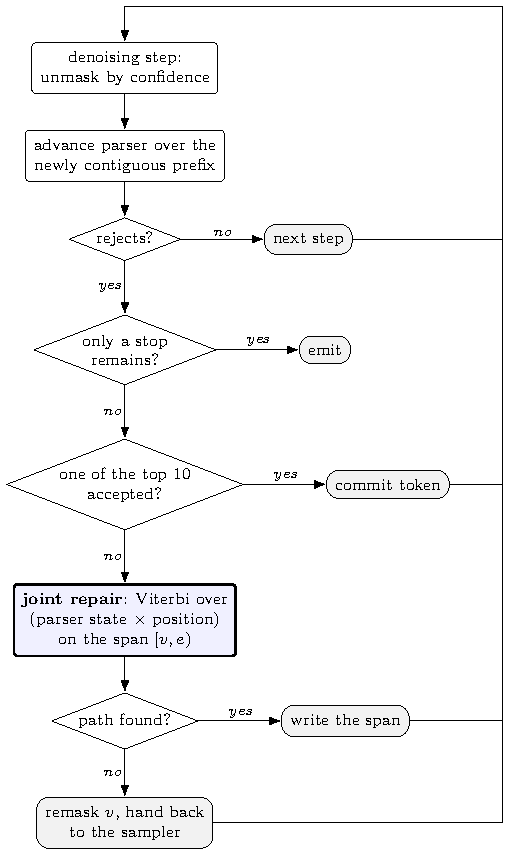
\includegraphics[width=0.52\linewidth]{pipeline.pdf}
\caption{Where the joint repair fires. Only a parser rejection reaches it, and
only after a stop test and a bounded retry have failed, so a clean step pays
nothing.}
\label{fig:pipeline}
\end{figure}

\section{The distribution of legal token sets}
\label{app:legalsets}

Section~\ref{sec:cand} rests on a claim about how many tokens an incremental
parser actually admits at a live state. This appendix gives the measurement and
the full distribution.

\paragraph{Procedure.}
We take the $40$ generated outputs of the DPGrammar run on JSONSchemaBench
\texttt{medium} (seed $0$, $T{=}128$) whose schemas compile, and replay each one
through \texttt{llguidance}~1.7.0 under teacher forcing: the parser is
initialised from the instance's schema, and the tokens the model actually
produced are fed to it one at a time. Before consuming each token we call
\texttt{compute\_logit\_bias()} and count the non-zero entries of the returned
mask; that count is $|\mathcal{L}(q)|$, the number of tokens the parser would
accept next. Replay stops at the first token the parser rejects, so every state
we record is one the decoder genuinely reached. This yields $6{,}657$ live
states over a vocabulary of $|V|=126{,}349$. The measurement is offline and
model-free, which needs only the schema and the emitted text, so it can be
reproduced without a GPU.

\paragraph{The distribution.}
Figure~\ref{fig:legalsets} shows the result. The distribution is not merely
skewed, it is bimodal: $38.4\%$ of states admit fewer than $100$ tokens
and $29.7\%$ admit more than $10{,}000$, leaving the decade between $10^4$ and
$10^5$ nearly empty. The median is $106$. The extremes are sharper still: before the first token
a JSON object grammar admits $2$ of $126{,}349$ tokens, and after the two
characters \texttt{\{\char34} it admits exactly one, the first character of
the only property name the schema allows there.

\begin{figure}[h]
\centering
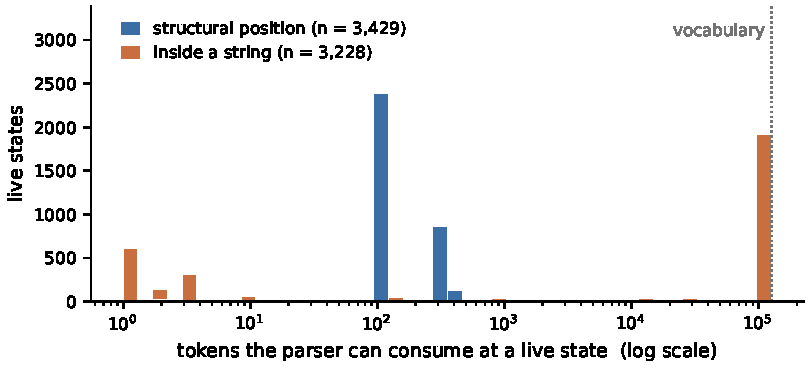
\includegraphics[width=0.86\linewidth]{legal_sets.pdf}
\caption{How many tokens an incremental parser admits, over $6{,}657$ live
states on JSONSchemaBench \texttt{medium} ($|V|=126{,}349$). The distribution is
bimodal and the decade between the modes is nearly empty, which is why no single
$k$ suits both. Structural positions are uniformly tight; the bimodality lives
inside strings, separating a partially spelled property name, which admits a
handful of continuations, from a free-form value, which admits almost the whole
vocabulary.}
\label{fig:legalsets}
\end{figure}

\paragraph{What the order of proposal and filter costs.}
The distribution above is why \S\ref{sec:cand} draws candidates from
$\mathcal{L}(q)$ rather than ranking $V$ and filtering. On \texttt{medium} the
admitted set is smaller than a top-$100$ draw at $38\%$ of live states, so a
filter-then-propose scheme is sampling against a small target at those
positions; conversely the set is smaller than $k$ at $40\%$ of state-positions,
where the edge set is enumerated exactly rather than sampled and the search at
that node is exhaustive rather than heuristic. Reversing the order in our own
implementation costs $1.2$\,pp of schema@1 and produces four repair sites where
the draw contained no token the parser would accept, a class the edge set cannot
produce (\S\ref{sec:ablation}).

\paragraph{Where the two modes come from.}
The obvious explanation, that the tight mode is structural punctuation and the
wide mode is string content, is only half right. Structural positions
($3{,}429$ states) are uniformly tight, with a median of $104$ and a quartile
range of $95$ to $324$. The bimodality lives entirely inside strings ($3{,}228$
states, p25 $=3$, median $=125{,}308$), where it separates two kinds of string:
a free-form value admits almost the whole vocabulary, whereas a partially
spelled property name admits a handful of continuations. Both modes matter for
repair. The wide one is where filtering a top-$k$ draw is wasteful but harmless;
the tight one is where it fails, and the tight one contains exactly the
positions a diffusion decoder is most likely to get wrong: key boundaries,
closings, and enumerated values.

\paragraph{When the automaton gives the complete candidate set.}
Where $|\mathcal{L}(q)| \le k$, Eq.~\ref{eq:cand} enumerates the edge set exactly rather
than sampling it, and the candidate set is provably complete:

\begin{center}
\small
\begin{tabular}{lrrrrrr}
\toprule
$k$ & $8$ & $32$ & $64$ & $100$ & $128$ & $256$ \\
\midrule
states with $|\mathcal{L}(q)| \le k$ & $16.4\%$ & $17.9\%$ & $18.1\%$ & $39.7\%$ & $54.0\%$ & $54.6\%$ \\
\bottomrule
\end{tabular}
\end{center}

The jump between $k{=}64$ and $k{=}128$ is the tight mode itself, which clusters
near $100$; this is why we set $k=100$ and why raising it further buys little.
The fraction varies widely across schemas (at $k{=}32$: median $18.4\%$,
interquartile range $9.8$--$28.3\%$, and $100\%$ for the most constrained schema
in the sample), so it is a property of the schema, not a constant of the
tokenizer.

\paragraph{Two facts the method depends on.}
First, no live state had an empty legal set ($0$ of $6{,}657$). This is what
makes the DP total: a live state always has a continuation, so the candidate set
is never empty and the search can always complete the span. Our termination rule
(\S\ref{sec:stop}) treats an empty mask as a failed read rather than as a stop
signal for this reason. Second, the mask read is cheap ($0.025$\,ms mean,
$0.012$\,ms median) and the implementation already performs it to compute the
state key used for path merging, so drawing candidates from the automaton adds
no parser calls beyond those already paid for.



\section{Ordering artifacts}
\label{app:ordering}

llguidance compiles a JSON schema into a grammar that fixes the order of an
object's properties to their declaration order: \texttt{\{"a":1,"b":2\}} is
rejected when the schema declares \texttt{b} first, although both orders satisfy
the schema and \texttt{jsonschema} accepts either. A model that writes the
properties in a different order therefore produces a violation that is not an
error, and the correct repair, moving a block, is not expressible by a
positional DP, which can only overwrite in place. The repair then writes the
demanded key name over a value intended for another field. We measured this class
at $7.6\%$ of $118$ violations; among the $16$ that occur where the grammar
admits exactly one token, half are of this kind.


\section{The parser interface}
\label{app:api}

The paper treats the incremental parser abstractly: a state $q$, a consumable
set $\mathcal{L}(q)$, and the ability to advance, copy, and undo. This appendix
records the concrete interface those abstractions are built on, so that the
method can be reimplemented against a different parser.

\paragraph{Construction.}
We use \textsc{llguidance}~1.7.0 \citep{microsoft2025llguidance}. A tokenizer is
built from the checkpoint's own \texttt{tokenizer.json}, so token boundaries in
the grammar and in the model agree exactly. A JSON Schema is compiled with
\texttt{grammar\_from\_json\_schema} and a SMILES grammar with
\texttt{grammar\_from\_lark}; compilation is checked before use, and a schema
that fails to compile is excluded from every arm rather than scored as a failure
for one (Table~\ref{tab:coverage} quantifies how many). We raise the default parser
limits to \texttt{max\_items\_in\_row}${=}20{,}000$ and
\texttt{step\_max\_items}${=}600{,}000$; at the defaults, deeply nested schemas
abort mid-parse.

\paragraph{The five operations.}
\begin{center}
\small
\begin{tabular}{lll}
\toprule
paper & \textsc{llguidance} & note \\
\midrule
$\mathcal{L}(q)$        & \texttt{compute\_logit\_bias()}    & byte mask over $V$; $0.025$\,ms mean \\
advance                 & \texttt{try\_consume\_tokens([t])} & returns tokens consumed; $0$ means rejected \\
copy a state            & \texttt{deep\_copy()}              & lattice nodes hold these \\
undo                    & \texttt{rollback(n)}               & probe without copying \\
may stop                & \texttt{is\_accepting()}           & state is final, not that it must stop \\
\bottomrule
\end{tabular}
\end{center}

\paragraph{Two details the method depends on.}
First, \textsc{eos} is marked legal by the bias at accepting states but is not a
consumable grammar symbol: \texttt{try\_consume\_tokens([\textsc{eos}])} returns
$0$ there. It is therefore excluded from the candidate set of
Eq.~\ref{eq:cand}: offering it wastes a slot, and where it is the only token the
bias marks legal it would empty the set and imitate a dead end. A termination rule written in terms of consumption would therefore
never fire, which is why \texttt{only\_stop\_remains} (\S\ref{sec:stop}) is
defined on the bias---nothing but stop tokens remains legal---rather than on
what the parser will consume. Second, the DP merges lattice paths on
\texttt{bytes}(\texttt{compute\_logit\_bias()}) as the state key: two parser
states that admit exactly the same tokens are indistinguishable to every
subsequent decision, so collapsing them is exact rather than an approximation.
The key is a value the implementation already computes to build the candidate
set, so merging costs no additional parser calls.




\section{Grammar coverage and the CD-CFG comparison}
\label{sec:coverage}

\begin{table}[t]
\centering
\small
\caption{Grammar coverage is a property of the compiler, not of the decoder.
Each arm inherits the schemas its toolchain accepts; validity is then measured
only on the $351$ \texttt{medium} schemas both toolchains compile, so the two
effects are not confounded.}
\label{tab:coverage}
\begin{tabular}{llcc}
\toprule
Method & Toolchain & Schemas compiled & Validity on the shared $351$ \\
\midrule
CD-CFG             & \textsc{rustformlang} & $383/586$ ($65.4\%$) & $45.0\%$ \\
LAVE               & \textsc{llguidance}   & $511/586$ ($87.2\%$) & $82.3\%$ \\
No-DP baseline     & \textsc{llguidance}   & $511/586$ ($87.2\%$) & $92.6\%$ \\
\textbf{DPGrammar} & \textsc{llguidance}   & $511/586$ ($87.2\%$) & $\mathbf{97.4\%}$ \\
\bottomrule
\end{tabular}
\end{table}

CD-CFG~\citep{cd4dllm} is run from the authors' released code, which builds its
constraint with \textsc{rustformlang}, the formal-language library distributed
in the same repository, rather than with
\textsc{llguidance}~\citep{microsoft2025llguidance}. The two
accept different schemas: $351$ compile under both, $160$ only under
\textsc{llguidance}, $32$ only under \textsc{rustformlang}, with
\textsc{rustformlang} rejecting $203$ of $586$ mostly over regular-expression
quantifiers that Python's \texttt{re} accepts.

Counting those $203$ as decoding failures would measure a regex front-end
rather than a decoding algorithm, so we report coverage separately and compare
decoding only on the shared $351$. There CD-CFG reaches $45.0\%$ validity with
$19$ timeouts against DPGrammar's $97.4\%$ with none, and the ordering of the
arms is unchanged from Table~\ref{tab:difficulty}. Every absolute value rises on
this subset, DPGrammar's from $96.7\%$ to $97.4\%$ and the no-DP baseline's from
$91.8\%$ to $92.6\%$, so the $160$ schemas only \textsc{llguidance} compiles are
the harder ones rather than the easier: restricting to what both front-ends
accept makes the task easier for every decoder, not just for CD-CFG.


\section{Where the extra wall time goes}
\label{app:workload}

DPGrammar is $3.3$\,s slower than the unrepaired baseline on \texttt{medium}.
Figure~\ref{fig:workload} attributes that difference to work rather than to a
time breakdown, because the instrumented counters cover only about a quarter of
wall clock in either arm.

\begin{figure}[h]
\centering
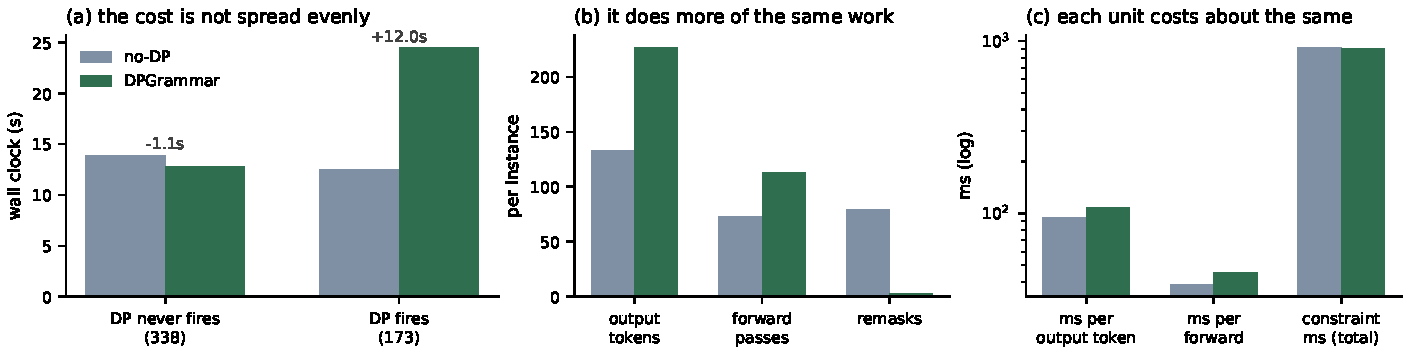
\includegraphics[width=\linewidth]{workload.pdf}
\caption{Averages per instance on JSONSchemaBench \texttt{medium}, split by
whether the repair layer ever fired. (a) The mean difference is concentrated in
the $173$ instances where it did; on the other $338$ the layer is slightly
faster. (b) On those instances it emits $71\%$ more tokens and needs
proportionally more forward passes, while remasking $28\times$ less. (c) Per
unit the two arms are close, and the constraint machinery costs the same in
both.}
\label{fig:workload}
\end{figure}

The bottleneck is not the search. The constraint machinery costs $909$\,ms
against the baseline's $920$, and grammar checks $22.5$\,ms against $11.2$. What
changes is how much gets written: the baseline stalls, remasking $79$ times and
stopping at $133$ tokens, while DPGrammar repairs and continues to $227$. That
takes $1.5\times$ the forward passes, each $1.2\times$ slower on the longer
sequence, which is the whole of the difference.

\section{Why validity alone is not enough}
\label{app:example}

Schema validity can be blind to a difference that matters, which is why
\S\ref{sec:metric} pairs it with a content floor rather than reporting it alone.
On \texttt{o78738} the schema asks for a course catalogue entry. Both arms
validate, so schema@1 scores them identically; what separates them is that the
unrepaired baseline stalls inside \texttt{prereqs}, emits two hundred lines of
whitespace, and closes the array empty:

\begin{center}
\footnotesize
\begin{minipage}{0.86\linewidth}
\begin{verbatim}
no-DP: valid, 4 populated leaves
[ { "code": "MATH 1001", "name": "Calculus I", "credits": "4",
    "description": "An introduction to calculus",
    "requirements": { "prereqs": [
                                       <200 lines of whitespace>
                      ], "coreqs": [] } } ]
\end{verbatim}
\end{minipage}
\end{center}

\noindent
DPGrammar reaches the same violation at position $120$, solves a three-position
span in which the parser admits fewer than two tokens on average, and the
decoder continues through the rest of the record:

\begin{center}
\footnotesize
\begin{minipage}{0.86\linewidth}
\begin{verbatim}
DPGrammar: valid, 12 populated leaves
[ { "code": "MATH 1001", "name": "Calculus I", "credits": "4",
    "description": "An introduction to calculus",
    "requirements": {
        "prereqs": [["MATH 0001", "MATH 0002"]],
        "coreqs":  [["MATH 1001", "MATH 1002"]] },
    "lectureHours": "3", "tutorialHours": "-", "labHours": "2",
    "note": "Recommended for first-year students" } ]
\end{verbatim}
\end{minipage}
\end{center}

\noindent
Neither output is wrong about the course; the baseline simply stops saying
anything, and validity cannot see the difference. Only the content floor
separates them, and it does so by $8$ populated leaves.

Neither instance is exceptional: across \texttt{medium}, $18.8\%$ of the
baseline's valid outputs carry fewer than five scalar leaves, against $12.1\%$
of ours.


\end{document}
